\chapter{Implementace algoritmu do GeoTools}
\label{chap:implementacealgoritmudogeotools}
	Pro implementaci polygonizačního algoritmu byla vybrána open-source knihovna pro programovací jazyk Java \textit{GeoTools}. V současné době je \textit{GeoTools} součástí \textit{OSGeo}, což je nezisková organizace, podporující open-source geoprostorové technologie. Mimo \textit{GeoTools} organizace zastupuje řadu dalších projektů, mezi které patří v desktopových aplikacích textit{QGIS}, \textit{GRASS GIS}, mezi mapové servery \textit{MapServer}, \textit{GeoServer} a mezi knihovnami jsou nejvýznamějšími zástupci \textit{GEOS}, \textit{GDAL}, \textit{PROJ}, nebo \textit{JTS}. Právě zmíněná knihovna \textit{JTS} tvoří základní kámen pro \textit{GeoTools}, jelikož jsou v ní definovány základní geometrické typy a operace pro práci s prostorovými daty. Možná více známá knihovna než \textit{JTS} je knihovna \textit{GEOS}, což je přepis knihovny z Javy do C++~\cite{OSGeo,GeoTools}.

\section{JTS Topology Suite}
	JTS je knihovna pro vytváření a manipulaci s vektorovou geometrií psaná v javě. Poskytuje nám řadu nástrojů pro práci s vektorovými daty, které budeme využívat při implementaci polygonizačního algoritmu, neimplementuje však například formáty pro uchování dat. JTS je šířena pod licencí BSD~\cite{locationtech}, která nám umožňuje knihovnu používat v podstatě bez omezení. Jedná se o jednu z nejsvobodnějších licencí.
	
\begin{figure}[h]
  \centering
  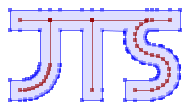
\includegraphics[width=5cm]{./pictures/7/jts_logo.png}
  \caption{Logo JTS Topology Suite. Převzato z \cite{locationtech}}
  \label{fig:7-jts}
\end{figure}
	
\section{GeoTools}
	GeoTools je toolkit pro práci s prostorovými daty, je šířen pod licencí LGPL, která nám umožňuje knihovnu využívat i v proprietárním softwaru, a však má své omezení pokud bysme měli v plánu vytvořit odvozené dílo. Datové struktury jsou založeny na specifikacích OGC, která poskytuje standardy pro geo prostorová data. Na obrázku \ref{fig:7-geotools} jsou znázorněny komponenty, ze kterých se geotools skládá. Je zde například vidět že GeoTools poskytuje sadu JTS. GeoTools využívá software jako například GeoServer, uDig, Geopublisher, Geomajas a mnoho dalších~\citep{GeoTools}.

	
\begin{figure}[h]
  \centering
  
\includegraphics[width=8cm]{./pictures/7/geotools_logo.png}
  \caption{Logo GeoTools. Převzato z \cite{GeoTools}.}
  \label{fig:7-geotools}
\end{figure}
	
	
\begin{figure}[h]
  \centering
  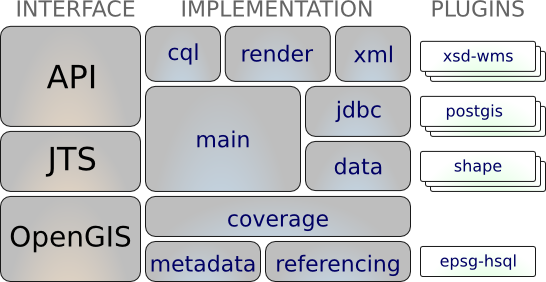
\includegraphics[width=10cm]{./pictures/7/geotools_struktura.png}
  \caption{Struktura GeoTools. Převzato z \cite{GeoTools}.}
  \label{fig:7-geotools}
\end{figure}
	
	
	
	
\section{GeoTools plug-in systém}
	Většina \textit{open-source} projektů je založena na příspěvcích od komunity vývojářu. Proto jsou projekty vytvořeny tak aby byli snadno rozšiřitelné o nějakou funkcionalitu. Výjimkou není ani projekt \textit{GeoTools}. Snaha vývojářů je tedy taková, co nejvíce usnadnit tvorbu zásuvných modulů. Na webových stránkách \textit{GeoTools}\cite{GeoTools} najdeme velmi podrobný tutoriál pro implementaci uživatelských funkcí a jiných dalších komponent. K tomuto účelu je využíváno technologie Java Service Provider Interface.
	
\subsection{Java Service Provider Interface}
	Java SPI přišla s nástupem Javy 6, která byla představena v roce 2006. Tato technologie umožňuje vyhledat a načíst implementaci daného rozhraní a tak dodat funkčnost. Této metody je využíváno například u přístupu k databázím pomocí JDBC, kdy třetí strana má možnost implementovat ovladače pro jakoukoli databázi a tak rozšířit funkčnost JDBC. Základními prvky SPI jsou:
	
\begin{itemize}
	\item Service
	\item Service provider interface
	\item Service provider
\end{itemize}	
	
\subsubsection{Service}
	Též hojně označované jako \textit{služba}. Jedná se o API se kterým programátor pracuje, aniž by věděl že 


\subsubsection{Service provider interface}
	Také nazývané \textit{rozhraní poskytovatele služeb}. Je rozhraní nebo abstraktní třída, která slouží jako koncový bod služby. Toto rozhraní nebo abstraktní třída je dále implementována poskytovatelem služeb.
	
	
\subsubsection{Service provider}
	V Češtině se někdy používá označení \textit{poskytovatel služeb} nebo zkráceně jen \textit{poskytovatel}. Jedná se o implementaci \textit{rozhraní poskytovatele služeb}. V analogii na \textit{JDBC} se může jednat o implementaci do konkrétní databáze.


\subsubsection{ServiceLoader class}




\subsection{Návrhový vzor Factory}



\subsection{První implementace}

	

